\section{问题重述}

\subsection{研究背景}

随着"双碳"战略的深入推进，新能源大规模并网消纳难的问题日益凸显。绿电直连项目作为促进新能源就近消纳的新路径，将风电、光伏等绿色电力直接供给本地用户，避免了远距离输电带来的损耗和调度困难。国家发展改革委、国家能源局发布的《关于有序推动绿电直连发展有关事项的通知》对绿电直连项目提出了明确的运行指标要求，包括新能源自发自用电量占总可用发电量比例大于60\%、总用电量绿电比例大于30\%、新能源上网电量占总可用发电量比例小于20\%等核心约束。

“绿电—绿氢—绿氨”一体化绿电直连化工园区正在成为解决新能源消纳和化工行业深度脱碳的重要路径。氨相较于氢更易于储运，因此以电解水制氢为中间环节、合成氨为终端产品的技术路线具有显著的工程应用价值。本文研究的绿电直连型电氢氨园区包含风力发电、光伏发电、碱性电解槽（ALKEL）、质子交换膜电解槽（PEMEL）、合成氨装置、储能设备及常规电负荷等核心组件，其运行优化涉及多时段功率调度、设备启停策略、储能配置等多维决策问题。

\subsection{问题概述}

本文针对绿电直连型电氢氨园区的优化运行问题，需要解决以下五个子问题：

（1）在典型风光场景下，假设电解槽与合成氨装置满负荷连续运行，基于功率平衡原则计算园区各项功率曲线和电量指标，分析绿电直连指标的满足情况及原因。

（2）将制氨产能扩容至72吨/日，在电氢氨装置仅有全额开机和停机两种运行方式的约束下，对5种产量水平分别求解成本最低的生产时段安排，并在24种风光场景下进行全年统计分析。

（3）在电氢氨装置功率连续可调（下限为10\%）的条件下，对24种风光场景求解最优功率调度方案，分析连续调节相对离散调节的改善效果。

（4）研究园区离网运行模式，在无储能和有储能两种条件下分析制氨产量和经济性，给出储能最优配置方案，并对比离网与联网两种运行模式的经济性。

（5）从电力系统运行角度，分析绿电直连园区容量渗透率显著提高后对电网的影响，并提出政策建议。

\begin{figure}[H]
\centering
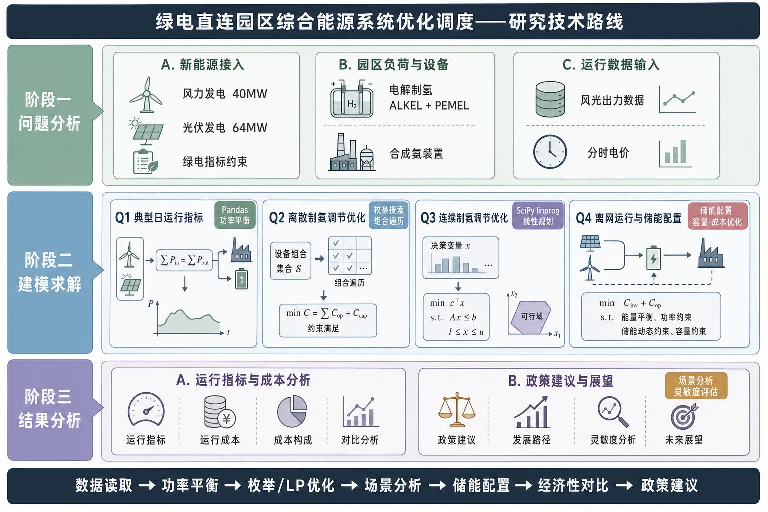
\includegraphics[width=\textwidth,height=0.45\textheight,keepaspectratio]{../figures/fig_roadmap.pdf}
\caption{整体技术路线图}\label{fig:roadmap}
\end{figure}

本文的整体技术路线如图\ref{fig:roadmap}所示，从问题一的基础指标计算出发，逐步深入到离散调节优化、连续调节优化、离网储能配置，最终上升到政策分析层面，形成了完整的研究体系。各子问题之间存在递进关系：问题一建立基础模型框架，问题二引入离散决策变量，问题三将决策空间从离散扩展到连续，问题四进一步去除电网支撑约束研究自治运行，问题五则从系统层面进行宏观分析。

\begin{figure}[H]
\centering
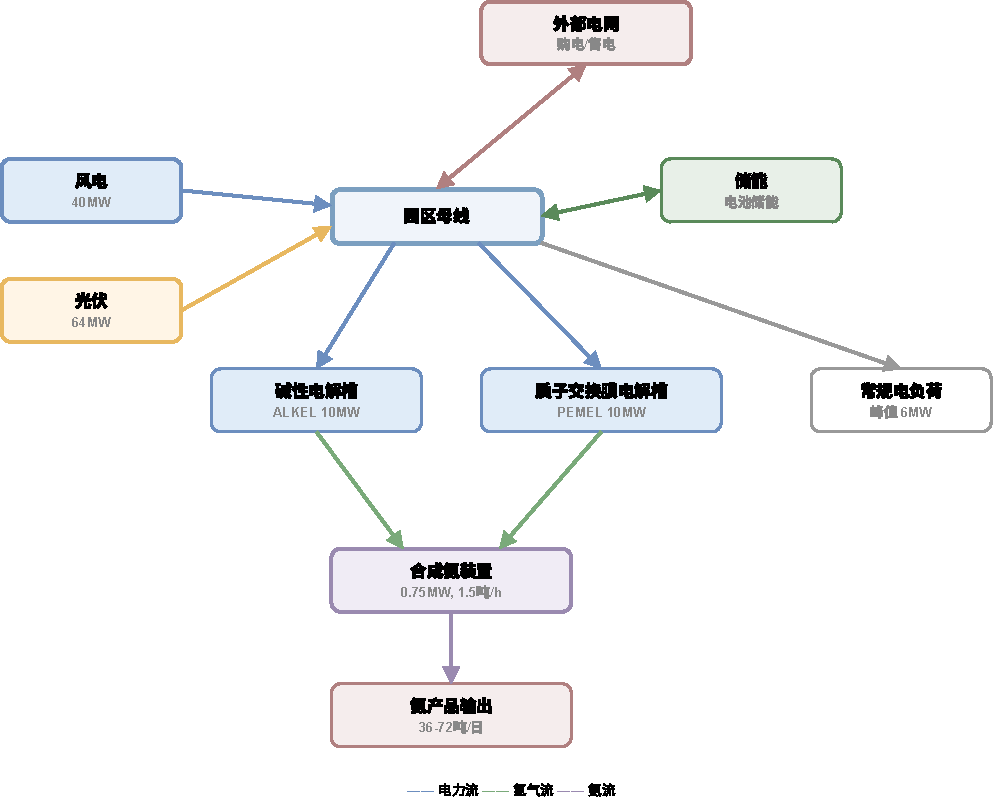
\includegraphics[width=0.9\textwidth,height=0.4\textheight,keepaspectratio]{../figures/fig_energy_topology.pdf}
\caption{绿电直连型电氢氨园区能量流拓扑图}\label{fig:energy_topology}
\end{figure}

园区的能量流拓扑结构如图\ref{fig:energy_topology}所示，风电和光伏作为绿色电力来源，通过直连方式供给碱性电解槽和质子交换膜电解槽进行电解水制氢，产出的氢气汇入合成氨装置生产氨产品。外部电网在联网模式下提供调峰备用服务，储能设备用于平衡风光波动。整个系统的核心特征是"绿电直连"，即风光发电不经过大电网调度直接连接用电设备，最大化绿电利用率。
